%% In this subsection, along with an outline of the work that you plan to do -- from
%% the start to the end of your project -- you should also indicate what you think
%% could possibly change as you embark on and continually work on your thesis. In
%% the outline of your work, you might want to describe your methods of data
%% collection, any hardware or software you plan to build or implement, or any
%% algorithms you design. Who you are and what you bring to your work will also
%% help define what you plan to do. Here I quote Professor Neil Spring quite
%% broadly:
%% 
%%   Provide personal insight [to your thesis proposal]. You undoubtedly have a
%%   different way of viewing the world than anyone else, perhaps more theoretical
%%   or practical or empirical or operational. Maybe you think more like a user or
%%   more like a software engineer. [Maybe you had an interesting internship or
%%   spend a summer abroad.] Perhaps your undergraduate minor shapes your
%%   worldview.
%% 
%%   Wherever this project leads you, it's what you bring to the process that
%%   makes it interesting for everyone else. Focus on techniques. Focus on the
%%   methods and how they can be applied to solve a problem. You can make an
%%   exception if conflicating or changing results motivate further analysis.
%%   Often the inputs (workload, applications, processor speeds, network speeds)
%%   will change, and so the results (performace, comparisons) and conclusions
%%   will change with them.
%% 
%% You should also indicate what kind of equipment, facilities, data, or other
%% material you may need for the completion of your work. It is imperative that
%% you provide a timeline or a clear schedule that indicates a plan for your
%% thesis work. In this plan you and your thesis supervisor should come to an
%% agreement on goals for each month of the project including (but not limited to)
%% experiments, data collection, analysis, any refining, drafting of thesis, final
%% results, and revision of thesis. You are welcome to insert a chart with a
%% summary of your goals for each month. Most EECS Master's degree theses are
%% assigned a total number of 360 hours. We ask that you plan accordingly.

\section{Proposed Work}

\subsection{Toolkit}

\todo[insert work from Nov-Jan in here]

\subsection{Dataset}

\begin{figure}[t]
    \centering
    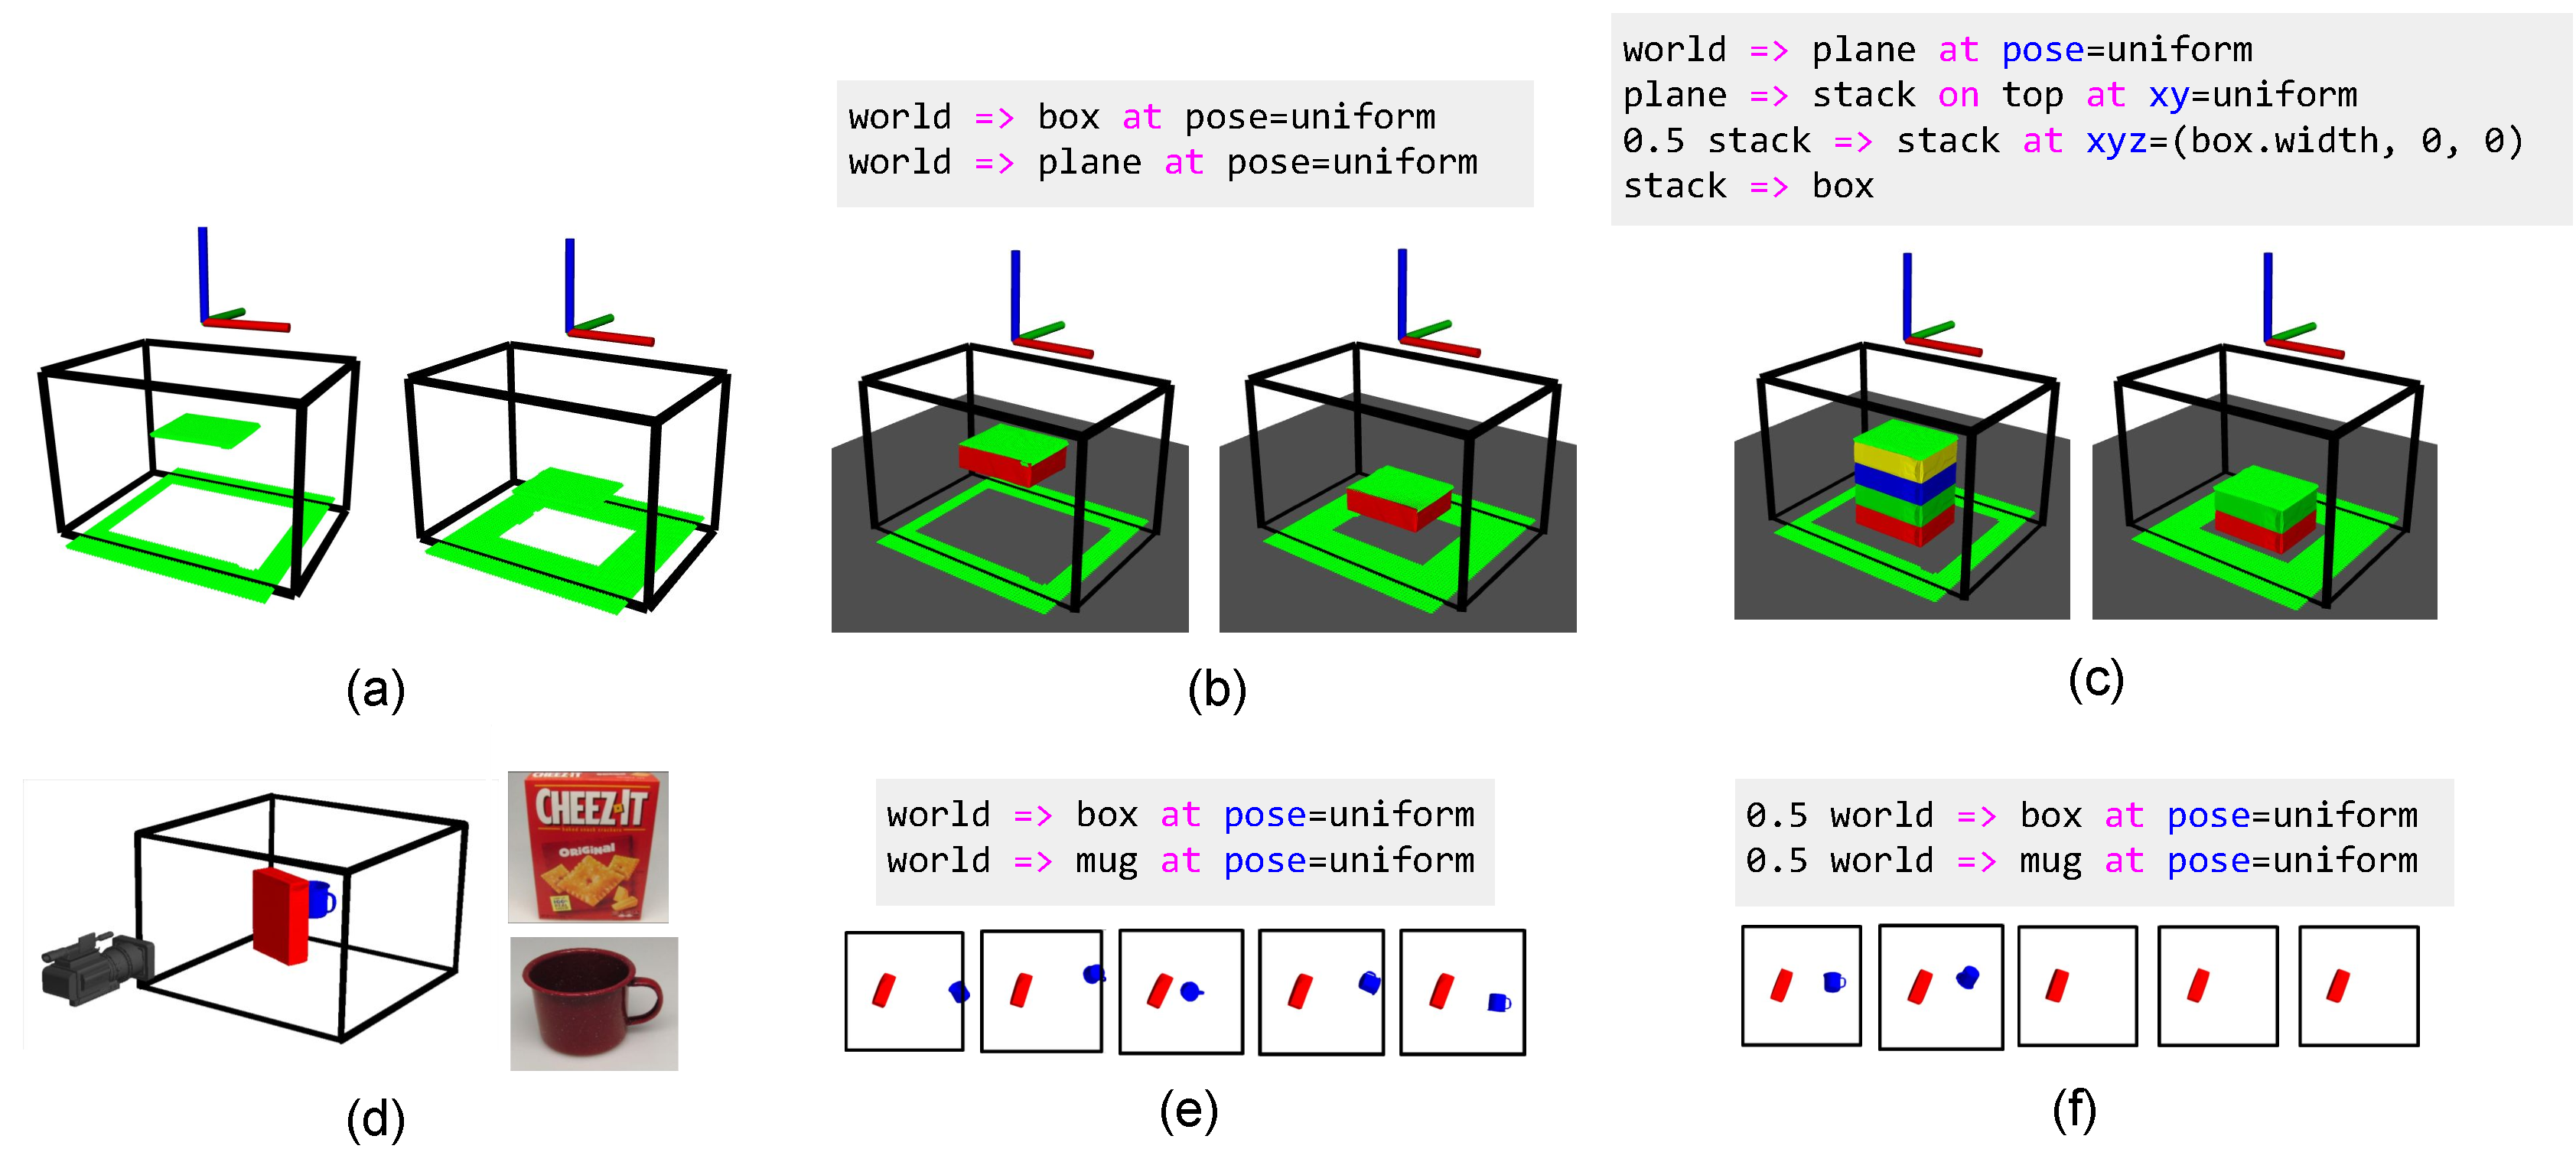
\includegraphics[width=\textwidth]{figures/lafi-fig.pdf}
    \caption{\small
Two scenarios with prior knowledge specified as programs in our probabilistic scene description language.
(a) shows two depth measurements made by a depth camera.
(b) shows a program in which boxes have random poses in 3D space, and the resulting inferred pose of the box.
(c) shows a program that assumes boxes are in stacks that rest on the floor, and the inferred number of boxes that explain the data for each observation.
(d) shows another scenario, where a depth camera observes a box that is occluding a mug.
(e) shows a program that asserts that both objects exist (but at unknown poses).
The resulting inferences show the mug must exist somewhere behind the box to be consistent with this knowledge and the observation.
(f) shows a program that allows for either object to not exist, and the resulting joint inferences about the mug's existence and pose.
}
    \label{fig:results}
\end{figure}

\todo[Insert current work from neurips and lafi. The dataset serves as a
simultaneous exploration of the research gap left by purely neural techniques,
and a series of preliminary solutions (perhaps both purely symbolic and
neuro-symbolic) that use Bayesian methods to address this gap.] \\

This part is a highly relevent research goal, due to the undervaluing of
semantic structuring of information by the neural network community. In some
sense we are trying to provide a solution to a problem that is not fully
visible to the community, or at the very least is thought to be "too hard" for
current techniques. Hard grounding metrics, or at least a fuller range of
explicitly specified common-sense tasks will go a long way in changing the
over-skeptical perspective toward Bayesian techniques trying to answer this
question. Thus, an important part of the thesis work will be identifying the
gap that exists between types of problems that we'd like to solve (common sense
reasoning), and how neural networks currently fail to address these problems,
as well as providing as much of a solution as we can in the time available,
which we believe will be compelling enough to demonstrate the utility of
Bayesian methods in modern CV pipelines.

\subsection{Neuro-Symbolic Predictive Coding OR Generative Modeling for Neuro-Predictive Error Correction}

In some ways the current state-of-the-art in both neural and probabilistic
techniques have orthogonal and complementary strengths and weaknesses. While
neural techniques exhibit strong performance in parsing out useful statistics
from massively high-dimensional data with relatively little compute, they
struggle to enforce semantically meaningful constraints on those statistics. On
the other hand, probabilistic techniques can naturally capture symbolic systems
and thus are much more expressible when it comes to representing and reasoning
about highly structured semantic content. However, the dominant paradigms for
inference treats it mostly as a top-down problem in which latent scene
parameters are estimated via mostly-blind random walks. This "guess-and-check"
methodology creates a bottleneck in propagating information from low-level
features to the statistics of interest.

We believe there is a natural road to combining the strength of these two
approaches. We propose a compositional technique where each system is used to
leverage its own abilities. We propose 

This corresponds to a meta-modeling predictive coding problem, in which we
represent and abstract the behavior of the black-box neural model with a
generative model that leverages the intuition we have about the failure modes
of these neural systems. Our generative procedure is not attempting to predict
the images themselves, but rather construct a robust model of the detector
itself in order to enrich the unstructured and noisy outputs of the detector
with structured information.

There is also a possible path to a more fully distributed set of models, via a
reformulation of the inference procedure as 

PROPOSED FIGURE: A spurious DOPE detection is pictured. Below, the abstract
scene graph is visualized, along with a percentage of occlusion. The more
abstract model captures this via increasing the uncertainty of the pose
estimation.
